\documentclass{article}
\usepackage[a4paper,margin=1in]{geometry}
\usepackage{tikz}
\usepackage[T1]{fontenc}
\usepackage[utf8]{inputenc}
\usepackage{lmodern}
\pagestyle{empty}

\usepackage{xfp}
\usepackage{xparse}

\NewDocumentEnvironment{timeline}{O{14} O{24} O{250} O{-3000} O{2025}}{% width, height, year step, start year, end year
  % Begin group
  \begingroup

  % Local variables
  \def\tlwidth{#1}%
  \def\tlheight{#2}%
  \def\tlyearstep{#3}%
  \def\tlstart{#4}%
  \def\tlend{#5}%
  \def\verticallinepos{0.5}%
  \pgfmathtruncatemacro{\tlsecondstep}{\tlstart + \tlyearstep}
  \pgfmathtruncatemacro{\numticks}{(\tlend - \tlstart)/\tlyearstep}

  \begin{tikzpicture}

  % Vertical axis
  \draw[very thick] (\verticallinepos,0) -- (\verticallinepos,\tlheight);
  \node[rotate=90] at (0, 0.5*\tlheight) {Time};

  % Loop from i = 0 to numticks
  \foreach \i in {0,...,\numticks} {
  % Compute current year
  \pgfmathtruncatemacro{\year}{\tlstart + \i * \tlyearstep}

  % Calculate position (float)
  \pgfmathsetmacro{\pos}{(\tlend - \year)/(\tlend - \tlstart) * \tlheight}

  % Only draw if pos is inside the bounds
  \pgfmathparse{(\pos >= 0) && (\pos <= \tlheight)}
  \ifnum\pgfmathresult>0
    % Prepare label
    \pgfmathtruncatemacro{\absyear}{abs(\year)}
    \ifnum\year<0
      \def\labeltext{\absyear~BCE}
    \else
      \def\labeltext{\absyear~CE}
    \fi

    % Draw the tick
    \draw[gray] (\verticallinepos,\pos) -- (\tlwidth,\pos) node[right] {\small \labeltext};
  \fi
  }

  % Define \timelineevent locally inside this environment
  \def\timelineevent##1##2##3##4{% year start, year end, name, distance from left line
    \pgfmathsetmacro{\ystart}{(\tlend - ##1)/(\tlend - \tlstart) * \tlheight}
    \pgfmathsetmacro{\yend}{(\tlend - ##2)/(\tlend - \tlstart) * \tlheight}
    \pgfmathsetmacro{\ytext}{(\ystart + \yend)/2}
    \draw[fill=yellow!50] (##4,\ystart) rectangle (##4+1,\yend);
    \node[rotate=90] at (##4+0.5,\ytext) {\tiny ##3};
  }%
}
{%
  \end{tikzpicture}
  \endgroup % End local scope
}

\begin{document}

\iffalse

Time line and chapter for:
Europe and Middle East;
Asia excluding Middle East;
Oceania;
Sub-Saharan Africa;
Americas;

%https://usefulcharts.com/products/timeline-of-world-history?srsltid=AfmBOopS9m5ZgO2ZgwRIQmrdXolLk8MB2rmKRCYCXRPoW1JgQ21a_9G0

I also want to include:
major bettles and events;
wide adoption of technology, like paper, printing press, computer...;


There should a environmets or command that simplifies creating the time lines.
The user should be able to define a time line where the user can start, stop, increase 
or decrease the time line or split it.
The user can speciy the coller and the text it should display.

Environment:
- fixed 15 column/timelines.
- The width of a timeline is given in mm
- The location/which column and start end is given in the timeline.
- If the time line need to change the column then a new time line needs to defined.
- To connect time lines you have "connect" or "transition" which is a dashed line.
- You can define a split given the start and finish.


\fi

aosfidjpowaiejfpoiejs fpoiasje oijespo ifjpoesai jpoijsa pofijesapoi jfpoifjpoiajf poiejsapo ijfpoifjpoijas pofijaspoijf poisa jfpoisajfpoijsa poijpoas ijpofijsa poifjsao ijpoijf paoijfpoeis japofijsa poijesaoifj oisaj poiajs poijfpoijsa poijas poijpsaoijfpoisa jfpoaiesjf poisaj poij sapoijf

%[12][20][-3000][2000]
\begin{timeline}
  \timelineevent{-3000}{-1000}{Ancient Egypt}{1}
  \timelineevent{1760}{1840}{Industrial Rev.}{4}
\end{timeline}


\newpage
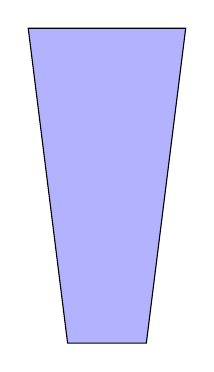
\begin{tikzpicture}
  % Narrow at bottom (x=0..1), wide at top (x=0..2), height=4
  \filldraw[fill=blue!30]
    (0.5,0) -- (1.5,0)     % bottom edge (width=1)
    -- (2,4) -- (0,4)  % top edge (width=2)
    -- cycle;
\end{tikzpicture}


\newpage
\begin{center}
\Large Timeline of World Empires (Scaled Dates)
\end{center}

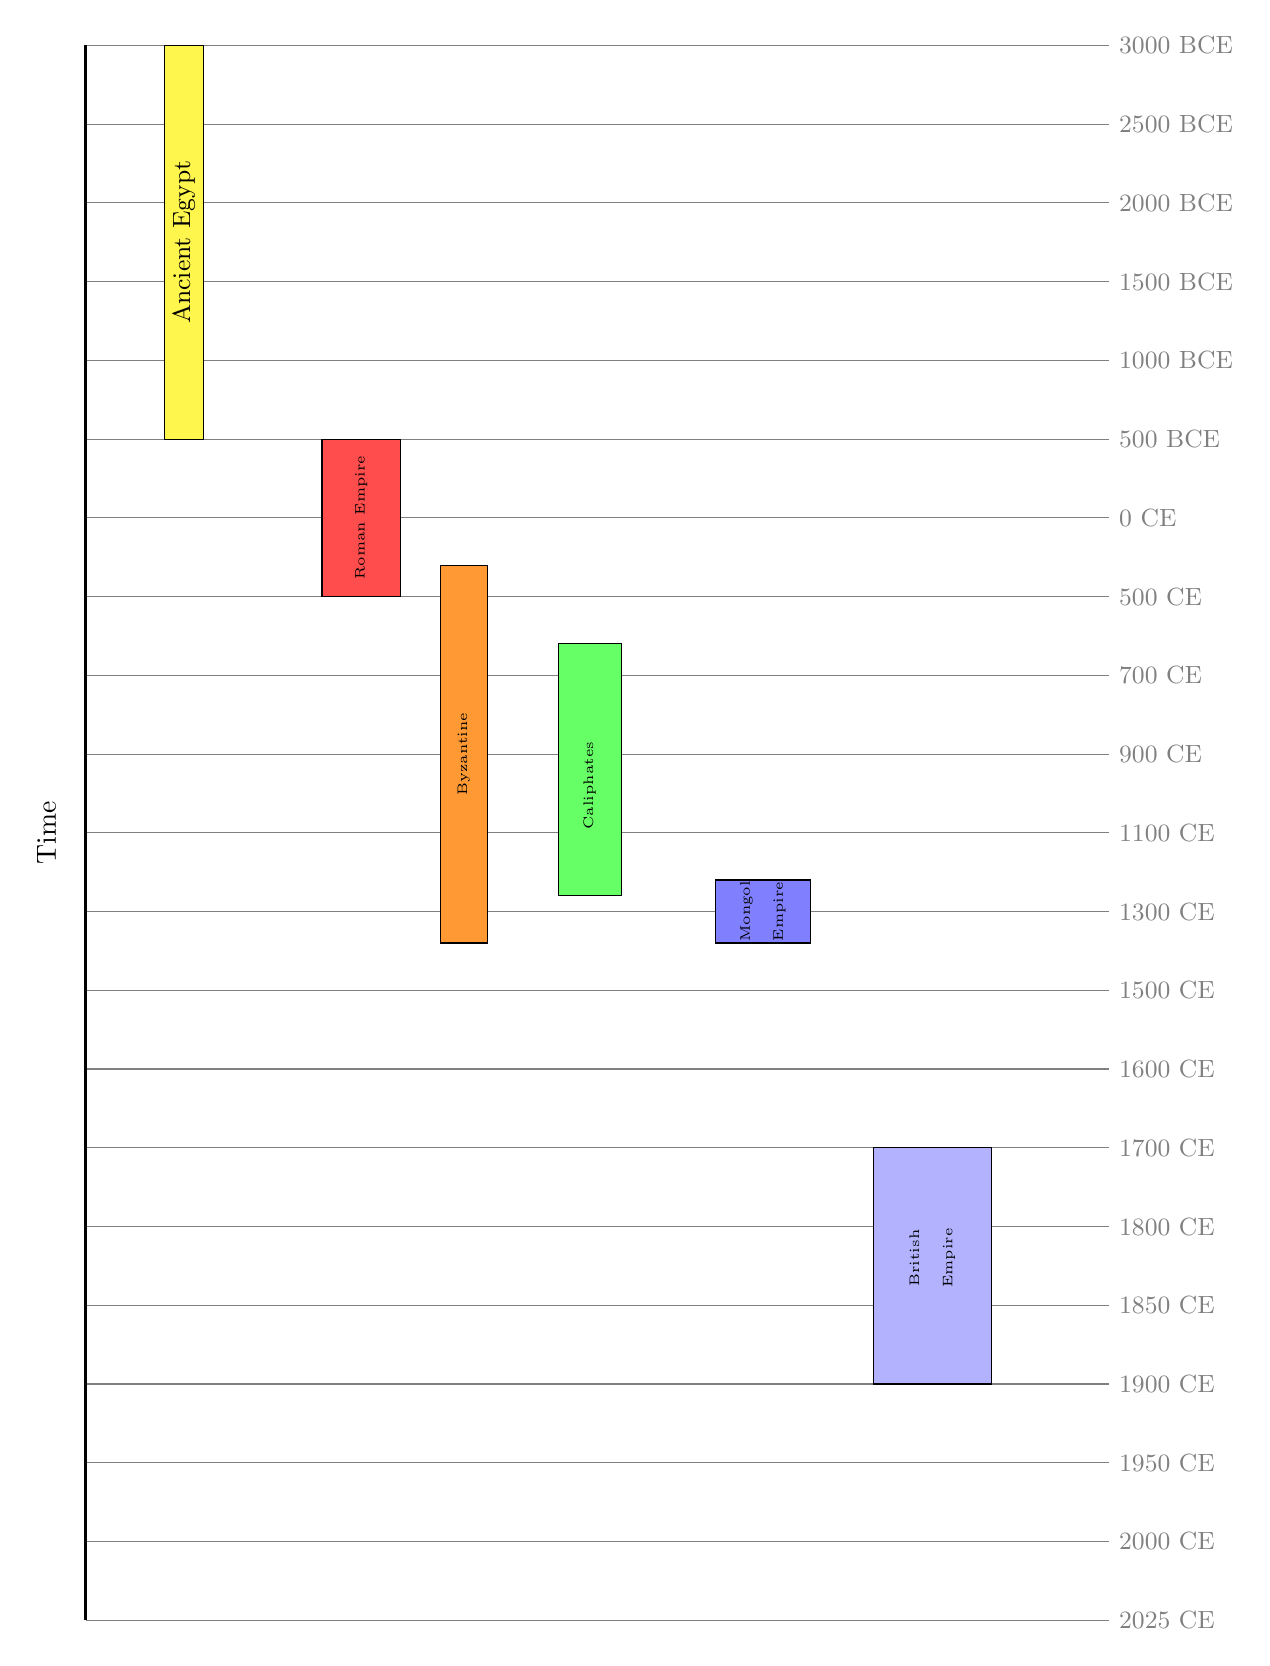
\begin{tikzpicture}[xscale=0.1, yscale=-0.2]

  % Draw year labels (scaled every 10 units = 500 years)
  \foreach \y/\label in {
    0/3000 BCE, 5/2500 BCE, 10/2000 BCE, 15/1500 BCE,
    20/1000 BCE, 25/500 BCE, 30/0 CE, 35/500 CE,
    40/700 CE, 45/900 CE, 50/1100 CE, 55/1300 CE,
    60/1500 CE, 65/1600 CE, 70/1700 CE, 75/1800 CE,
    80/1850 CE, 85/1900 CE, 90/1950 CE, 95/2000 CE,
    100/2025 CE}
    \draw[gray] (0,\y) -- (130,\y) node[right] {\small \label};

  % Timeline vertical line
  \draw[very thick] (0,0) -- (0,100);
  \node[rotate=90] at (-5, 50) {Time};

  % Empires (Y = (year + 3000) / 50)

  % Ancient Egypt: -3000 to -500 → Y = 0 to 25
  \draw[fill=yellow!70] (10,0) rectangle (15,25);
  \node[rotate=90] at (12.5,12.5) {\small Ancient Egypt};

  % Roman Empire: -500 to 500 → Y = 25 to 35
  \draw[fill=red!70] (30,25) rectangle (40,35);
  \node[rotate=90] at (35,30) {\tiny Roman Empire};

  % Byzantine Empire: 300 to 1453 → Y = 33 to 57
  \draw[fill=orange!80] (45,33) rectangle (51,57);
  \node[rotate=90] at (48,45) {\tiny Byzantine};

  % Caliphates: 650–1258 → Y = 38 to 54
  \draw[fill=green!60] (60,38) rectangle (68,54);
  \node[rotate=90] at (64,47) {\tiny Caliphates};

  % Mongol Empire: 1206–1368 → Y = 53 to 57
  \draw[fill=blue!50] (80,53) rectangle (92,57);
  \node[rotate=90, align=center] at (86,55) {\tiny Mongol \\ \tiny Empire};

  % British Empire: 1700–1900 → Y = 70 to 85
  \draw[fill=blue!30] (100,70) rectangle (115,85);
  \node[rotate=90, align=center] at (107.5,77) {\tiny British \\ \tiny Empire};

\end{tikzpicture}

\end{document}

